\section{Methodologies}\label{sec:methodologies}
Just like \poke evolve upon reaching certain conditions, we applied the same reasoning for the development of our bot. First of all we started with a simple player (called \textit{MaxBasePower} or \textit{MBP}) that chooses the non-status move with the highest base power, regardless of the actual damage dealt. Then, we upgraded this first simple player by letting it choose the move with the highest actual damage thanks to a hand-crafted stats and damage computations (we called this player as \textit{BestDamage} or \textit{BD}).

The damage computation is the main engine of our bot, since the more accurate is the damage dealt the higher the performance of the players.

\begin{multline} 
    damage = \left (\frac{(\frac{2\times level}{5} + 2) \times power \times A/D}{50} + 2 \right) \\ \times targets \times PB \times weather \times critical \\ \times random \times STAB \times type \times burn \times other
\label{eq:damage}   
\end{multline}

As we can see from \eqref{eq:damage}, the damage computation is made up of many parameters and each one of them contains several rules that can be explained in FOL, an example is shown in \eqref{eq:rule}.
\begin{multline}
    \forall x \hspace{1mm} \poke(x) \wedge \forall y \hspace{1mm} Move(y) \wedge Holds(x,airbaloon) \\
    \wedge MoveType(y,Ground) \Rightarrow Immune(x,y)
    \label{eq:rule}
\end{multline}

After finishing the engine, we had to deal with switches; the main issue with them is that there is not an optimal number and the situations in which we should use this mechanic can not be hard-coded since they would be too many. To alleviate all of this, we decided to build what we have called a \textit{matchup} function that, given the two \poke, computes the advantage (or disadvantage) the bot has. The computation of the \textit{matchup} value for each not fainted bot's \poke is based on the damage multipliers coming from their types and moves:
\begin{enumerate}
    \item First we take the max damage multiplier based on types for both the bot's and opponent's \poke as shown in \autoref{fig:damage_multipliers}.
    \item Then, we compute the difference between the two values obtaining what we called the \textit{type advantage}.
    \item We do the same for the moves, in case the opponent's \poke has no known moves we suppose that it will have at least one move for each one of its types and we assign it a default move.
    \item Just like we did for the types we do the same difference to compute the \textit{move advantage}
    \item At the end, we sum both values to obtain the actual \textit{matchup} $\in [-8,8]$ which indicates how favourable is the current situation for the bot's \poke against the opponent's.
\end{enumerate}
\begin{figure}[!htbp]
    \centering
    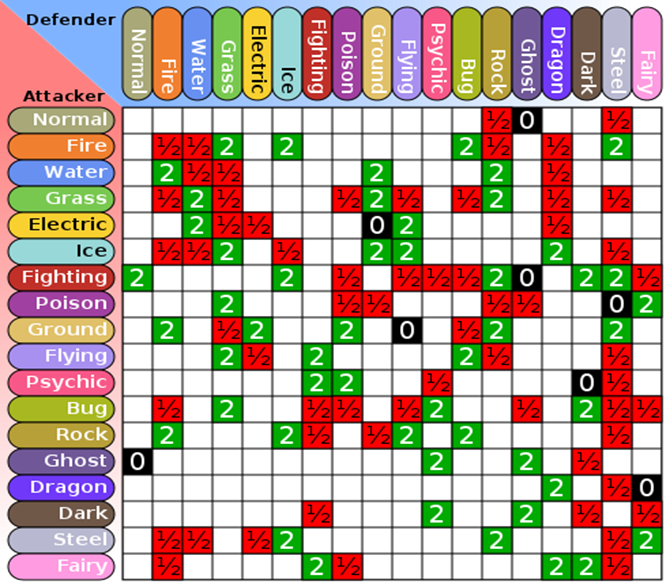
\includegraphics[width=0.8\linewidth]{images/damage_multipliers.png}
    \caption{Damage multipliers for each type}
    \label{fig:damage_multipliers}
\end{figure}

\subsection{Rule-Based Player}\label{subsec:rule_based_player}
The first enhanced version of our bot is the rule-based player (or \textit{RB}) which uses everything we talked about until now plus some more improvements thanks to an external expert. We defined even more rules to deal with \textit{healing}, \textit{status}, \textit{boost}, \textit{protective} and \textit{retaliatory} moves, while also implementing a strategy for deciding when to switch out and under which situations we should use the gimmick, which is dynamax for the generation our bot will play in.

\subsection{MiniMax Player}\label{subsec:minimax_player}
The second enhanced player we developed uses the minimax algorithm with $\alpha$-$\beta$ pruning in order to choose the best action to take (we called such player as \textit{MiniMax} or \textit{MM}). Generally, a player can choose either to make a move or to switch out the active \textit{Pokémon}, for this reason, the mini-max tree has a branching factor that is the sum of the number of available moves of the active \poke and the number of available switches; the latter are, usually, the number of not fainted \poke in a team.

The root node of a tree represents the actual current state of a battle that we want to start simulating, in which we assume the bot to take an action first i.e. before the opponent player. The depth of the tree is two time the turns we want to simulate because in a \poke battle, a turn ends when both the players have chosen an action. In this way, assuming $t$ is the turn we want to simulate, the effects of our actions are computed at each $2t + 1$ depth level, while the opponent ones at every $2t$, with $t>0$, depth level. Taking into account everything we have seen until now we can say that each one of the nodes simulates the progress of a battle, as an example, see \autoref{fig:minimax_with_switches}.

As we first said in \autoref{sec:introduction}, a \poke battle is a partially observable environment in which the opponent’s team, \poke statistics, abilities and moves can not be known a priori and each move has its own probability to hit. As a consequence, the library \cite{poke_env} does not allow to simulate the progress of a battle, otherwise it would have been like cheating. To overcome these limitations, at the beginning of each battle, we build a knowledge base that is composed by the \poke that belong to our team and all their attributes plus the opponent's active \textit{Pokémon}. Whenever the opponent player chooses a move or switches to a \textit{Pokémon}, we add these information to the knowledge base in order to simulate the progress of the battle more accurately as possible. It is not possible to consider all the variables of a battle, so the most relevant ones we considered are: the weather conditions, the moves, statistics and boosts of both active \poke and finally, the composition of our team and the opponent's. All these variables may change from turn to turn assuming a crucial role when computing the damage, the recoil or the drain of a move. Then, in order to know whether or not we are at an advantage over the opponent, we developed an heuristic.

\subsection{Heuristic}\label{subsec:heuristic}
To estimate the utility of a node, we use an heuristic that uses knowledge of the current state to tell us how favourable is a particular battle progress.

Initially, we used a straightforward evaluation function that uses only the knowledge of both active \poke: we considered the ratio of the current hp (health points) of the \poke over its max hp \eqref{eq:simple_heuristic}.
\begin{multline}
    f(node)=\bar{hp}\left(active_{Bot}\right)-\bar{hp}\left(active_{Opp}\right)
    \label{eq:simple_heuristic}
\end{multline}
The minimax algorithm with such function has some limitations since it has no global knowledge about the state of the game: as an example, the opponent's active \poke might be defeated, but all the remaining \poke of his team are alive; in this case, the rating function gives a very positive score even if our team has only one not fainted \poke.

Considering these limits, we decided to use a more reliable function that considers the ratio between the hp of the entire team and the number of surviving \poke. Finally, we added a penalty term on the depth of the node to the evaluation function \cite{showdown_competition}; this penalty promotes exploration among all possible strategies and discourages excessive turn depth.
The resulting evaluation function is a linear weighted sum \eqref{eq:complex_heuristic} where the weight of each term indicates how relevant the term is to the state evaluation. By defying $alive(team)= num \; of \; \text{\textit{Pokémon}} \; alive \; in \; the \; team$, the evaluation function can be written as:

\begin{equation}
\begin{split}
    f(node)&=w_1 \cdot \bar{hp}(team_{Bot}) +w_2 \cdot alive\left(team_{Bot}\right) \\ 
    & - w_3 \cdot \bar{hp}\left(team_{Opp}\right)
    - w_4 \cdot alive\left(team_{Opp}\right) \\
    &-w_5 \cdot depth(node)
\end{split}
\label{eq:complex_heuristic}
\end{equation}
We performed a random search on the weights to find the best configuration of the function and evaluated each configuration by observing the minimax player's performances. The best-resulting weights configuration favours dealing damage to the opposing Pokemon rather than rewarding survival and associates a small depth penalty.
